\documentclass[12pt]{article}
\usepackage{graphicx,import}
\usepackage[svgnames]{xcolor} 
\usepackage{fancyhdr}
\usepackage{subfig}
\usepackage{hyperref}
\usepackage{enumitem}
\usepackage{cite}
\usepackage[many]{tcolorbox}
\usepackage{listings }
\usepackage[a4paper, total={6in, 8in} , bottom = 25mm , top = 25mm, headheight = 1.25cm , includehead,includefoot,heightrounded ]{geometry}
\usepackage{afterpage}
\usepackage{amssymb}
\usepackage{pdflscape}
\usepackage{gensymb}
\usepackage{textcomp}
\usepackage{tikz,pgfplots}
\usepackage{xecolor}
\usepackage{rotating}
\usepackage{pdfpages}
\usepackage{fancyvrb}
\usepackage[Kashida]{xepersian}
\usepackage[T1]{fontenc}
\usepackage{tikz}
\usepackage[utf8]{inputenc}
\usepackage{PTSerif} 
\usepackage{seqsplit}

\usepackage[edges]{forest}

\usepackage{listings}
\usepackage{xcolor}

\hypersetup{
	colorlinks   = true, %Colours links instead of ugly boxes
	urlcolor     = blue, %Colour for external hyperlinks
	linkcolor    = blue, %Colour of internal links
	citecolor   = red %Colour of citations
}

\definecolor{codegreen}{rgb}{0,0.6,0}
\definecolor{codegray}{rgb}{0.5,0.5,0.5}
\definecolor{codepurple}{rgb}{0.58,0,0.82}
\definecolor{backcolour}{rgb}{0.95,0.95,0.92}

\NewDocumentCommand{\codeword}{v}{
	\texttt{\textcolor{blue}{#1}}
}
\lstset{language=java,keywordstyle={\bfseries \color{blue}}}

\lstdefinestyle{mystyle}{
	backgroundcolor=\color{backcolour},   
	commentstyle=\color{codegreen},
	keywordstyle=\color{magenta},
	numberstyle=\tiny\color{codegray},
	stringstyle=\color{codepurple},
	basicstyle=\ttfamily\normalsize,
	breakatwhitespace=false,         
	breaklines=true,                 
	captionpos=b,                    
	keepspaces=true,                 
	numbers=left,                    
	numbersep=5pt,                  
	showspaces=false,                
	showstringspaces=false,
	showtabs=false,                  
	tabsize=2
}

\lstset{style=mystyle}

\settextfont[Scale=1.2 ,BoldFont={Bahij Nazanin-Bold.ttf} , ItalicFont = {IRNazaninIranic.ttf}]{Bahij Nazanin-Regular.ttf}
\setlatintextfont[Scale = 1.0]{Garamond}
\DefaultMathsDigits 
\DeclareMathSizes{11}{19}{13}{9} 
%\DeclareMathSizes{12}{14.4}{8}{9}





\newenvironment{changemargin}[2]{%
	\begin{list}{}{%
			\setlength{\topsep}{0pt}%
			\setlength{\leftmargin}{#1}%
			\setlength{\rightmargin}{#2}%
			\setlength{\listparindent}{\parindent}%
			\setlength{\itemindent}{\parindent}%
			\setlength{\parsep}{\parskip}%
		}%
		\item[]}{\end{list}}


\definecolor{foldercolor}{RGB}{124,166,198}

\tikzset{pics/folder/.style={code={%
			\node[inner sep=0pt, minimum size=#1](-foldericon){};
			\node[folder style, inner sep=0pt, minimum width=0.3*#1, minimum height=0.6*#1, above right, xshift=0.05*#1] at (-foldericon.west){};
			\node[folder style, inner sep=0pt, minimum size=#1] at (-foldericon.center){};}
	},
	pics/folder/.default={20pt},
	folder style/.style={draw=foldercolor!80!black,top color=foldercolor!40,bottom color=foldercolor}
}

\forestset{is file/.style={edge path'/.expanded={%
			([xshift=\forestregister{folder indent}]!u.parent anchor) |- (.child anchor)},
		inner sep=1pt},
	this folder size/.style={edge path'/.expanded={%
			([xshift=\forestregister{folder indent}]!u.parent anchor) |- (.child anchor) pic[solid]{folder=#1}}, inner xsep=0.6*#1},
	folder tree indent/.style={before computing xy={l=#1}},
	folder icons/.style={folder, this folder size=#1, folder tree indent=3*#1},
	folder icons/.default={12pt},
}

\begin{document}
	
	
	%%% title pages
	\begin{titlepage}
		\begin{center}
			
			\vspace*{0.7cm}
			
			
\includegraphics[width=0.4\textwidth]{sharif1.png}\\
			\vspace{0.5cm}
			\textbf{ \Huge{\emph  ﺷﺒﻜﻪ‌های کامپیوتری} }\\
			\vspace{0.5cm}
			\textbf{ \Large{ تمرین دوم - سوال سوم} }
			\vspace{0.2cm}
			
			
			\large \textbf{دانشکده مهندسی کامپیوتر}\\\vspace{0.2cm}
			\large   دانشگاه صنعتی شریف\\\vspace{0.2cm}
			\large   ﻧﯿﻢ سال دوم 00-99 \\\vspace{0.2cm}
			\noindent\rule[1ex]{\linewidth}{1pt}
			استاد:\\
			\textbf{{جناب آقای دکتر جعفری}}
			
			
			\vspace{0.15cm}
			نام و نام خانوادگی:\\
			
			
			\textbf{{امیرمهدی نامجو - 97107212}}
		\end{center}
	\end{titlepage}
	%%% title pages
	
	
	%%% header of pages
	\newpage
	\pagestyle{fancy}
	\fancyhf{}
	\fancyfoot{}
	\cfoot{\thepage}
	\chead{تمرین دوم}
	\rhead{
\includegraphics[width=0.1\textwidth]{sharif.png}}
	\lhead{امیرمهدی نامجو}
	%%% header of pages
	


\newpage
\section*{سوال سوم}

\begin{enumerate}
	\item 
	بعد از اجرای اسکریپت پایتون، دستورات زیر را اجرا می‌کنیم:
	
	\begin{latin}
	\begin{lstlisting}[language=bash]
		xterm h1 h3
	\end{lstlisting}
\end{latin}

با \lr{\Verb+ifconfig+} متوجه‌ می‌شویم که IP هاست اول \lr{\Verb+10.0.0.1+} است.

دستور زیر را در هاست اول اجرا می‌کنیم:
	
\begin{latin}
	\begin{lstlisting}[language=bash]
		iperf3 -s
	\end{lstlisting}
\end{latin}

و در هاست سوم دستور زیر را اجرا می‌کنیم:
\begin{latin}
	\begin{lstlisting}[language=bash]
		iperf3 -c 10.0.0.1 -t 10
	\end{lstlisting}
\end{latin}

\begin{latin}
	\begin{Verbatim}
Connecting to host 10.0.0.1, port 5201
[  6] local 10.0.0.3 port 47408 connected to 10.0.0.1 port 5201
[ ID] Interval           Transfer     Bandwidth       Retr  Cwnd
[  6]   0.00-1.00   sec  2.42 MBytes  20.3 Mbits/sec    0   31.1 KBytes       
[  6]   1.00-2.00   sec  2.24 MBytes  18.8 Mbits/sec    0   31.1 KBytes       
[  6]   2.00-3.00   sec  2.24 MBytes  18.8 Mbits/sec    0   31.1 KBytes       
[  6]   3.00-4.00   sec  2.24 MBytes  18.7 Mbits/sec    0   31.1 KBytes       
[  6]   4.00-5.00   sec  2.24 MBytes  18.8 Mbits/sec    0   31.1 KBytes       
[  6]   5.00-6.00   sec  2.17 MBytes  18.2 Mbits/sec    0   31.1 KBytes       
[  6]   6.00-7.00   sec  2.30 MBytes  19.3 Mbits/sec    0   31.1 KBytes       
[  6]   7.00-8.00   sec  2.11 MBytes  17.7 Mbits/sec    0   31.1 KBytes       
[  6]   8.00-9.00   sec  2.30 MBytes  19.3 Mbits/sec    0   31.1 KBytes       
[  6]   9.00-10.00  sec  2.17 MBytes  18.3 Mbits/sec    0   31.1 KBytes       
- - - - - - - - - - - - - - - - - - - - - - - - -
[ ID] Interval           Transfer     Bandwidth       Retr
[  6]   0.00-10.00  sec  22.4 MBytes  18.8 Mbits/sec    0             sender
[  6]   0.00-10.00  sec  22.3 MBytes  18.7 Mbits/sec                  receiver
	
		
	\end{Verbatim}
\end{latin}

همان طور که مشاهده‌ می‌شود، گذردهی نهایی \lr{\Verb+18.8 Mbits/sec+} گزارش شده است. چیزی که انتظار داریم در اصل $20$ است اما این عدد هم تفاوت چندانی ندارد.  دلیل این تفاوت می‌تواند به این مربوط باشد که در این جا عملا یک سوییچ واقعی شبیه سازی شده است و یکسری پارامترهای درونی خود پروتکل \lr{OpenFlow1.3} تاثیر گذار بوده‌اند. مخصوصا در قسمت‌های بعدی شاهد تفاوت‌های جدی‌تری خواهیم بود که آن ها را بهتر می‌توان توجیه کرد. 

ضمنا اعداد بالا تا حد خوبی برای هر دو طرف یکسان هستند و تفاوت معناداری بین‌‌ آن‌ها مشاهده نمی‌شود.

\item
دستورات مشابهی را مانند بالا برای هاست اول و دوم اجرا می‌کنیم.

نتایج برای هر کدام از طرفین متفاوت است. برای فرستنده:


\begin{latin}
	\begin{Verbatim}
[  6] local 10.0.0.2 port 43558 connected to 10.0.0.1 port 5201
[ ID] Interval           Transfer     Bandwidth       Retr  Cwnd
[  6]   0.00-1.00   sec   362 KBytes  2.96 Mbits/sec    0    110 KBytes       
[  6]   1.00-2.00   sec  7.36 MBytes  61.7 Mbits/sec    0   1.38 MBytes       
[  6]   2.00-3.00   sec  3.75 MBytes  31.5 Mbits/sec    0   1.91 MBytes       
[  6]   3.00-4.00   sec  2.50 MBytes  21.0 Mbits/sec    0   2.02 MBytes       
[  6]   4.00-5.00   sec  2.50 MBytes  21.0 Mbits/sec    0   2.14 MBytes       
[  6]   5.00-6.00   sec  2.50 MBytes  21.0 Mbits/sec    0   2.25 MBytes       
[  6]   6.00-7.00   sec  2.50 MBytes  21.0 Mbits/sec    0   2.36 MBytes       
[  6]   7.00-8.00   sec  2.50 MBytes  21.0 Mbits/sec    0   2.48 MBytes       
[  6]   8.00-9.00   sec  2.50 MBytes  21.0 Mbits/sec    0   2.58 MBytes       
[  6]   9.00-10.00  sec  2.50 MBytes  21.0 Mbits/sec    0   2.69 MBytes       
- - - - - - - - - - - - - - - - - - - - - - - - -
[ ID] Interval           Transfer     Bandwidth       Retr
[  6]   0.00-10.00  sec  29.0 MBytes  24.3 Mbits/sec    0             sender
[  6]   0.00-10.00  sec  21.9 MBytes  18.4 Mbits/sec                 receiver
		
		
		
		
	\end{Verbatim}
\end{latin}

اما در سمت گیرنده شاهد چنین اعداد هستیم:

\begin{latin}
	\begin{Verbatim}
[  7] local 10.0.0.1 port 5201 connected to 10.0.0.2 port 43558
[ ID] Interval           Transfer     Bandwidth
[  7]   0.00-1.00   sec  82.0 KBytes   672 Kbits/sec                  
[  7]   1.00-2.00   sec  1.27 MBytes  10.7 Mbits/sec                  
[  7]   2.00-3.00   sec  2.27 MBytes  19.0 Mbits/sec                  
[  7]   3.00-4.00   sec  2.27 MBytes  19.0 Mbits/sec                  
[  7]   4.00-5.00   sec  2.27 MBytes  19.0 Mbits/sec                  
[  7]   5.00-6.00   sec  2.27 MBytes  19.0 Mbits/sec                  
[  7]   6.00-7.00   sec  2.27 MBytes  19.1 Mbits/sec                  
[  7]   7.00-8.00   sec  2.27 MBytes  19.0 Mbits/sec                  
[  7]   8.00-9.00   sec  1.97 MBytes  16.5 Mbits/sec                  
[  7]   9.00-10.00  sec  2.27 MBytes  19.0 Mbits/sec                  
[  7]  10.00-11.03  sec   662 KBytes  5.27 Mbits/sec                  
[  7]  11.03-12.37  sec  38.2 KBytes   233 Kbits/sec                  
[  7]  12.37-13.37  sec  80.6 KBytes   658 Kbits/sec                  
[  7]  13.37-14.37  sec   628 KBytes  5.18 Mbits/sec                  
[  7]  14.37-15.37  sec  17.0 KBytes   139 Kbits/sec                  
[  7]  15.37-16.37  sec  17.0 KBytes   138 Kbits/sec                  
[  7]  16.37-17.04  sec   105 KBytes  1.28 Mbits/sec                  
[  7]  17.04-18.03  sec   116 KBytes   963 Kbits/sec                  
[  7]  18.03-19.36  sec  46.7 KBytes   287 Kbits/sec                  
[  7]  19.36-20.36  sec  11.3 KBytes  92.7 Kbits/sec                  
[  7]  20.36-21.22  sec  91.9 KBytes   882 Kbits/sec                  
[  7]  21.22-22.36  sec  74.9 KBytes   537 Kbits/sec                  
[  7]  22.36-23.36  sec  18.4 KBytes   151 Kbits/sec                  
[  7]  23.36-24.36  sec   109 KBytes   891 Kbits/sec                  
[  7]  24.36-25.36  sec  15.6 KBytes   128 Kbits/sec                  
[  7]  25.36-26.36  sec  60.8 KBytes   499 Kbits/sec                  
[  7]  26.36-26.82  sec   679 KBytes  12.0 Mbits/sec                  
- - - - - - - - - - - - - - - - - - - - - - - - -
[ ID] Interval           Transfer     Bandwidth       Retr
[  7]   0.00-26.82  sec  29.0 MBytes  9.06 Mbits/sec    0             sender
[  7]   0.00-26.82  sec  21.9 MBytes  6.85 Mbits/sec                  receiver

	\end{Verbatim}
\end{latin}

مشاهده می‌کنیم که در سمت دریافت کننده اعداد \lr{Throughput} بسیار کمتر هستند. دلیل این موضوع به دلیل \lr{Latency} موجود در شبکه است. این موضوع باعث شده که بسته ها دیرتر به مقصد برسند و به علاوه شاهد تغییرات جدی در \lr{Congestion Window} سمت فرستنده هم هستیم.

اثر اصلی \lr{Latency} در این است که باعث می‌شود که Ack ها به موقع دریافت نشوند.

در حالت قبلی RTT کمتر از $1ms$ بود و تنها موضوعی که گلوگاه بود، سرعت خود لینک بود ولی در این جا RTT حدود $200ms$ است و این موضوع گلوگاه ایجاد کرده است.

\item


با اجرای دستورات مشابه، نتیجه زیر را داریم:

\begin{latin}
	\begin{Verbatim}

[  6] local 10.0.0.5 port 47704 connected to 10.0.0.4 port 5201
[ ID] Interval           Transfer     Bandwidth       Retr  Cwnd
[  6]   0.00-1.00   sec  2.16 MBytes  18.0 Mbits/sec   22   11.3 KBytes       
[  6]   1.00-2.00   sec  1.12 MBytes  9.36 Mbits/sec   12   9.90 KBytes       
[  6]   2.00-3.00   sec  1018 KBytes  8.38 Mbits/sec    4   11.3 KBytes       
[  6]   3.00-4.00   sec   891 KBytes  7.30 Mbits/sec    4   9.90 KBytes       
[  6]   4.00-5.00   sec  1018 KBytes  8.34 Mbits/sec    2   12.7 KBytes       
[  6]   5.00-6.00   sec   891 KBytes  7.29 Mbits/sec   12   9.90 KBytes       
[  6]   6.00-7.00   sec   764 KBytes  6.26 Mbits/sec    3   11.3 KBytes       
[  6]   7.00-8.00   sec  1018 KBytes  8.33 Mbits/sec    5   9.90 KBytes       
[  6]   8.00-9.00   sec  1.99 MBytes  16.7 Mbits/sec   18   14.1 KBytes       
[  6]   9.00-10.00  sec  2.24 MBytes  18.8 Mbits/sec   13   17.0 KBytes       
- - - - - - - - - - - - - - - - - - - - - - - - -
[ ID] Interval           Transfer     Bandwidth       Retr
[  6]   0.00-10.00  sec  13.0 MBytes  10.9 Mbits/sec   95             sender
[  6]   0.00-10.00  sec  12.8 MBytes  10.7 Mbits/sec                  receiver


	\end{Verbatim}
\end{latin}


برای سمت دیگر هم به همین شکل است. مشاهده‌ می‌کنیم که گذردهی و Bandwidth حدودا نصف شده است. 
در اصل Loss به دو شکل تاثیر گذار است. از یک سو نیاز به ارسال مجدد بسته‌های از دست رفته داریم. از سوی دیگر Cwnd نمی‌تواند به حالت بهینه ثابتی دست یابد. به علاوه تاثیر مستقیم آن‌هم این است که دیتایی که از دست رفته باشد را عملا نمی‌توان در Throughput به حساب آورد و همین موضوع هم موجب گذردهی می‌شود.


\item

سه رقم آخر $212$ است.

هاست چهارم را سرور می‌کنیم.

\begin{latin}
	\begin{lstlisting}[language=bash]
		iperf3 -s
	\end{lstlisting}
\end{latin}

و از هاست اول به آن داده ارسال می‌کنیم.

$$212 MB = 222298112 Byte$$


\begin{latin}
	\begin{lstlisting}[language=bash]
		 iperf3 -c 10.0.0.4 -J>result.json -n 222298112 
	\end{lstlisting}
\end{latin}

خروجی نهایی برای سمت گیرنده بدین شکل است:

\begin{latin}
\begin{Verbatim}
[  7] local 10.0.0.4 port 5201 connected to 10.0.0.1 port 39646
[ ID] Interval           Transfer     Bitrate
[  7]   0.00-1.00   sec  2.10 MBytes  17.6 Mbits/sec                  
[  7]   1.00-2.00   sec  2.25 MBytes  18.9 Mbits/sec                  
[  7]   2.00-3.00   sec  2.24 MBytes  18.8 Mbits/sec                  
[  7]   3.00-4.00   sec  2.25 MBytes  18.9 Mbits/sec                  
[  7]   4.00-5.00   sec  2.26 MBytes  18.9 Mbits/sec                  
[  7]   5.00-6.00   sec  2.26 MBytes  18.9 Mbits/sec                  
[  7]   6.00-7.00   sec  2.25 MBytes  18.9 Mbits/sec                  
[  7]   7.00-8.00   sec  2.25 MBytes  18.8 Mbits/sec                  
[  7]   8.00-9.00   sec  2.25 MBytes  18.8 Mbits/sec                  
[  7]   9.00-10.00  sec  2.24 MBytes  18.8 Mbits/sec                  
[  7]  10.00-11.00  sec  2.25 MBytes  18.8 Mbits/sec                  
[  7]  11.00-12.00  sec  2.25 MBytes  18.9 Mbits/sec                  
[  7]  12.00-13.00  sec  2.24 MBytes  18.8 Mbits/sec                  
[  7]  13.00-14.00  sec  2.23 MBytes  18.7 Mbits/sec                  
[  7]  14.00-15.00  sec  2.24 MBytes  18.8 Mbits/sec                  
[  7]  15.00-16.00  sec  2.25 MBytes  18.9 Mbits/sec                  
[  7]  16.00-17.00  sec  2.23 MBytes  18.7 Mbits/sec                  
[  7]  17.00-18.00  sec  2.25 MBytes  18.9 Mbits/sec                  
[  7]  18.00-19.00  sec  2.25 MBytes  18.9 Mbits/sec                  
[  7]  19.00-20.00  sec  93.3 KBytes   764 Kbits/sec                  
[  7]  20.00-21.00  sec  67.9 KBytes   556 Kbits/sec                  
[  7]  21.00-22.00  sec  5.41 MBytes  45.4 Mbits/sec                  
[  7]  22.00-23.00  sec   946 KBytes  7.74 Mbits/sec                  
[  7]  23.00-24.00  sec  1.35 MBytes  11.3 Mbits/sec                  
[  7]  24.00-25.00  sec  2.26 MBytes  18.9 Mbits/sec                  
[  7]  25.00-26.00  sec  2.26 MBytes  18.9 Mbits/sec                  
[  7]  26.00-27.00  sec  2.26 MBytes  18.9 Mbits/sec                  
[  7]  27.00-28.00  sec  2.26 MBytes  18.9 Mbits/sec                  
[  7]  28.00-29.00  sec  2.25 MBytes  18.9 Mbits/sec                  
[  7]  29.00-30.01  sec   949 KBytes  7.73 Mbits/sec                  
[  7]  30.01-31.00  sec   567 KBytes  4.67 Mbits/sec                  
[  7]  31.00-32.00  sec  1.48 MBytes  12.4 Mbits/sec                  
[  7]  32.00-33.00  sec  1.33 MBytes  11.2 Mbits/sec                  
[  7]  33.00-34.00  sec  1.46 MBytes  12.2 Mbits/sec                  
[  7]  34.00-35.00  sec  2.24 MBytes  18.8 Mbits/sec                  
[  7]  35.00-36.00  sec  1.69 MBytes  14.2 Mbits/sec                  
[  7]  36.00-37.00  sec  1.93 MBytes  16.2 Mbits/sec                  
[  7]  37.00-38.00  sec  2.25 MBytes  18.8 Mbits/sec                  
[  7]  38.00-39.00  sec  2.26 MBytes  19.0 Mbits/sec                  
[  7]  39.00-40.00  sec  1.65 MBytes  13.8 Mbits/sec                  
[  7]  40.00-41.00  sec  2.25 MBytes  18.9 Mbits/sec                  
[  7]  41.00-42.00  sec   711 KBytes  5.83 Mbits/sec                  
[  7]  42.00-43.00  sec  1.93 MBytes  16.2 Mbits/sec                  
[  7]  43.00-44.00  sec  1.82 MBytes  15.2 Mbits/sec                  
[  7]  44.00-45.00  sec  0.00 Bytes  0.00 bits/sec                  
[  7]  45.00-46.00  sec   624 KBytes  5.11 Mbits/sec                  
[  7]  46.00-47.00  sec   805 KBytes  6.59 Mbits/sec                  
[  7]  47.00-48.00  sec  7.79 MBytes  65.3 Mbits/sec                  
[  7]  48.00-49.00  sec  2.24 MBytes  18.8 Mbits/sec                  
[  7]  49.00-50.00  sec  1.87 MBytes  15.7 Mbits/sec                  
[  7]  50.00-51.00  sec  1.80 MBytes  15.1 Mbits/sec                  
[  7]  51.00-52.00  sec  2.26 MBytes  18.9 Mbits/sec                  
[  7]  52.00-53.00  sec  2.10 MBytes  17.6 Mbits/sec                  
[  7]  53.00-54.00  sec  2.26 MBytes  19.0 Mbits/sec                  
[  7]  54.00-55.00  sec  1.01 MBytes  8.44 Mbits/sec                  
[  7]  55.00-56.00  sec  1.53 MBytes  12.9 Mbits/sec                  
[  7]  56.00-57.01  sec  1.78 MBytes  14.8 Mbits/sec                  
[  7]  57.01-58.00  sec  1.38 MBytes  11.7 Mbits/sec                  
[  7]  58.00-59.00  sec  2.19 MBytes  18.3 Mbits/sec                  
[  7]  59.00-60.00  sec  2.13 MBytes  17.9 Mbits/sec                  
[  7]  60.00-61.00  sec  1.74 MBytes  14.6 Mbits/sec                  
[  7]  61.00-62.01  sec  1.32 MBytes  11.0 Mbits/sec                  
[  7]  62.01-63.00  sec  2.13 MBytes  18.0 Mbits/sec                  
[  7]  63.00-64.00  sec  1.87 MBytes  15.7 Mbits/sec                  
[  7]  64.00-65.00  sec  1.93 MBytes  16.2 Mbits/sec                  
[  7]  65.00-66.00  sec  1.92 MBytes  16.1 Mbits/sec                  
[  7]  66.00-67.00  sec  2.19 MBytes  18.4 Mbits/sec                  
[  7]  67.00-68.00  sec  1.70 MBytes  14.2 Mbits/sec                  
[  7]  68.00-69.00  sec  2.26 MBytes  18.9 Mbits/sec                  
[  7]  69.00-70.00  sec  1.73 MBytes  14.6 Mbits/sec                  
[  7]  70.00-71.00  sec  0.00 Bytes  0.00 bits/sec                  
[  7]  71.00-72.00  sec   115 KBytes   938 Kbits/sec                  
[  7]  72.00-73.00  sec  2.92 MBytes  24.5 Mbits/sec                  
[  7]  73.00-74.00  sec  6.10 MBytes  51.2 Mbits/sec                  
[  7]  74.00-75.00  sec  2.26 MBytes  18.9 Mbits/sec                  
[  7]  75.00-76.00  sec  1.69 MBytes  14.2 Mbits/sec                  
[  7]  76.00-77.00  sec  1.93 MBytes  16.2 Mbits/sec                  
[  7]  77.00-78.00  sec  2.26 MBytes  19.0 Mbits/sec                  
[  7]  78.00-79.01  sec   983 KBytes  7.94 Mbits/sec                  
[  7]  79.01-80.01  sec  1.38 MBytes  11.7 Mbits/sec                  
[  7]  80.01-81.01  sec   641 KBytes  5.26 Mbits/sec                  
[  7]  81.01-82.00  sec  1.23 MBytes  10.4 Mbits/sec                  
[  7]  82.00-83.00  sec  1.56 MBytes  13.1 Mbits/sec                  
[  7]  83.00-84.00  sec  2.05 MBytes  17.2 Mbits/sec                  
[  7]  84.00-85.00  sec  1.47 MBytes  12.4 Mbits/sec                  
[  7]  85.00-86.01  sec  1.96 MBytes  16.3 Mbits/sec                  
[  7]  86.01-87.00  sec  1.71 MBytes  14.5 Mbits/sec                  
[  7]  87.00-88.00  sec  1.93 MBytes  16.2 Mbits/sec                  
[  7]  88.00-89.00  sec  1.97 MBytes  16.5 Mbits/sec                  
[  7]  89.00-90.00  sec  1.19 MBytes  10.0 Mbits/sec                  
[  7]  90.00-91.00  sec  2.04 MBytes  17.1 Mbits/sec                  
[  7]  91.00-92.00  sec  1.97 MBytes  16.5 Mbits/sec                  
[  7]  92.00-93.00  sec  2.26 MBytes  19.0 Mbits/sec                  
[  7]  93.00-94.00  sec  2.25 MBytes  18.9 Mbits/sec                  
[  7]  94.00-95.01  sec  1.23 MBytes  10.2 Mbits/sec                  
[  7]  95.01-96.00  sec  2.03 MBytes  17.2 Mbits/sec                  
[  7]  96.00-97.00  sec   708 KBytes  5.80 Mbits/sec                  
[  7]  97.00-98.00  sec   264 KBytes  2.17 Mbits/sec                  
[  7]  98.00-99.00  sec  1.07 MBytes  8.96 Mbits/sec                  
[  7]  99.00-100.00 sec  6.93 MBytes  58.1 Mbits/sec                  
[  7] 100.00-101.00 sec  2.24 MBytes  18.8 Mbits/sec                  
[  7] 101.00-102.00 sec  2.24 MBytes  18.8 Mbits/sec                  
[  7] 102.00-103.00 sec  2.25 MBytes  18.8 Mbits/sec                  
[  7] 103.00-104.00 sec  1.88 MBytes  15.7 Mbits/sec                  
[  7] 104.00-105.32 sec   238 KBytes  1.48 Mbits/sec                  
[  7] 105.32-106.33 sec   100 KBytes   818 Kbits/sec                  
[  7] 106.33-107.32 sec   246 KBytes  2.02 Mbits/sec                  
[  7] 107.32-108.33 sec  29.7 KBytes   242 Kbits/sec                  
[  7] 108.33-109.32 sec  25.5 KBytes   210 Kbits/sec                  
[  7] 109.32-110.32 sec   290 KBytes  2.38 Mbits/sec                  
[  7] 110.32-111.32 sec  14.1 KBytes   116 Kbits/sec                  
[  7] 111.32-112.34 sec  52.3 KBytes   423 Kbits/sec                  
[  7] 112.34-113.32 sec   233 KBytes  1.94 Mbits/sec                  
[  7] 113.32-114.32 sec  12.7 KBytes   104 Kbits/sec                  
[  7] 114.32-115.32 sec  28.3 KBytes   232 Kbits/sec                  
[  7] 115.32-116.32 sec  14.1 KBytes   116 Kbits/sec                  
[  7] 116.32-117.32 sec   151 KBytes  1.24 Mbits/sec                  
[  7] 117.32-118.32 sec  19.8 KBytes   162 Kbits/sec                  
[  7] 118.32-119.31 sec  43.8 KBytes   360 Kbits/sec                  
[  7] 119.31-120.31 sec   228 KBytes  1.87 Mbits/sec                  
[  7] 120.31-120.33 sec  8.48 KBytes  4.39 Mbits/sec                  
- - - - - - - - - - - - - - - - - - - - - - - - -
[ ID] Interval           Transfer     Bitrate
[  7]   0.00-120.33 sec   203 MBytes  14.2 Mbits/sec                  receiver


\end{Verbatim}
\end{latin}

حال باید به کمک داده‌های فایل Json که در سمت فرستنده ایجاد شده نمودارها را ایجاد کنیم.

\begin{center}
	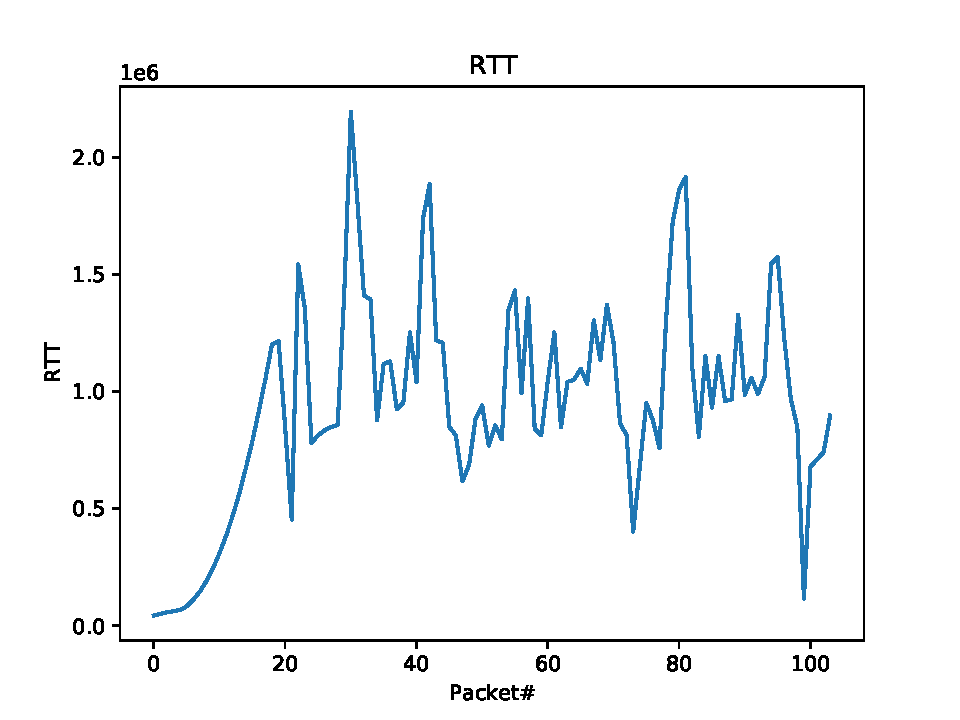
\includegraphics[page=1, width = 0.6 \textwidth]{images/plots.pdf}
\end{center}

\begin{center}
	\includegraphics[page=2, width = 0.6 \textwidth]{images/plots.pdf}
\end{center}

\begin{center}
	\includegraphics[page=3, width = 0.6 \textwidth]{images/plots.pdf}
\end{center}

\end{enumerate}
\end{document}



